\chapter{Regression}
\label{ch:capitolo4}
Different regression techniques were applied to the dataset, testing
on different combinations of attributes. The target variable chosen for
Univariate and Multiple regression was \texttt{criticReviewsTotal}, while
for Multivariate regression, the target variables were both
\texttt{userReviewsTotal} and \texttt{criticReviewsTotal}.
These were chosen because they offer important insights into the engagement
that a product can generate, which also was the focus of the binary
classification task in section~\ref{sec:binary_classification}.


\section{Univariate and Multiple Regression}
For Univariate Regression, the attribute
\texttt{criticReviewsTotal} was chosen
as the target variable. Aside from the semantic meaning, this choice was also made
because it has a high correlation
with the attribute \texttt{userReviewsTotal}, allowing univariate regression
to be performed, while maintaining a clear separate semantic meaning.
Figure~\ref{fig:univariate_regression} shows the results of the Univariate Regression task for
all models but KNN, which doesn't provide an interesting visualization.
\begin{figure}[H]
    \centering
    \begin{subfigure}{0.2565\textwidth}
        \centering
        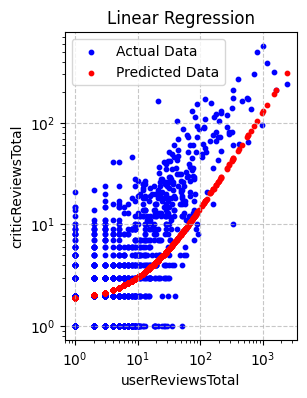
\includegraphics[width=1\textwidth]{plots/linear.png}
        \caption{Linear regressor}
        \captionsetup{width=0.9\linewidth, justification=centering}
        \label{fig:linear}
    \end{subfigure}
    \begin{subfigure}{0.24\textwidth}
        \centering
        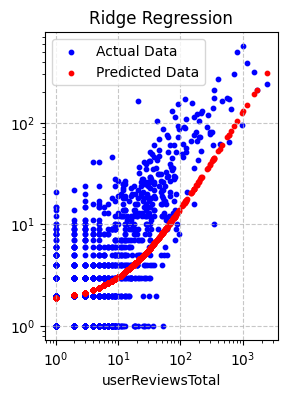
\includegraphics[width=1\textwidth]{plots/ridge.png}
        \caption{Ridge regressor}
        \captionsetup{width=0.9\linewidth, justification=centering}
        \label{fig:ridge}
    \end{subfigure}
    \begin{subfigure}{0.24\textwidth}
        \centering
        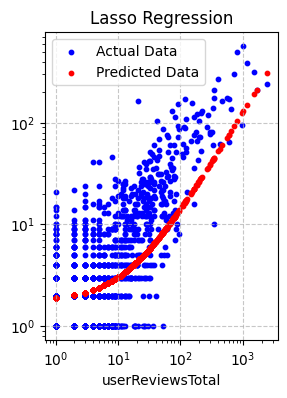
\includegraphics[width=1\textwidth]{plots/lasso.png}
        \caption{Lasso regressor}
        \captionsetup{width=0.9\linewidth, justification=centering}
        \label{fig:lasso}
    \end{subfigure}
    \begin{subfigure}{0.24\textwidth}
        \centering
        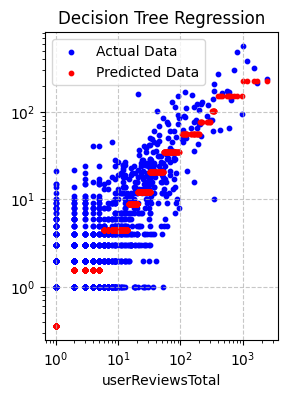
\includegraphics[width=1\textwidth]{plots/dt_regressor.png}
        \caption{DT regressor}
        \captionsetup{width=0.9\linewidth, justification=centering}
        \label{fig:elastic}
    \end{subfigure}
    \caption{Univariate regression prediction results in Logarithmic space}
    \label{fig:univariate_regression}
\end{figure}

\begin{table}[H]
    \centering
    \begin{tabular}{lcccccccc}
        \toprule
        % mae, mse normalized over target variable range
         & \textbf{Intercept} & \textbf{Coefficient} & \textbf{MAE} & \textbf{MSE} & \textbf{R$^2$} & \textbf{test MAE} & \textbf{test MSE} \\
        \midrule
        \textbf{Univariate} & & & & & \\
        \midrule
        Linear & 1.76 & 0.13 & 0.007 & 0.25 & 0.36 & 0.007 & 0.33 \\
        Ridge & 1.76 & 0.13 & 0.007 & 0.25 & 0.36 & 0.007 & 0.33 \\
        Lasso & 1.76 & 0.13 & 0.007 & 0.25 & 0.36 & 0.007 & 0.33 \\
        DT & - & - & 0.005 & 0.12 & 0.69 & 0.004 & 0.19 \\
        20-NN & - & - & 0.005 & 0.14 & 0.66 & 0.004 & 0.22 \\
        \midrule
        \textbf{Multiple} & & & & & \\
        \midrule
        Linear & - & - & 0.000 & 0.000 & 1.000 \\
        Ridge & - & - & 0.000 & 0.000 & 1.000 \\
        Lasso & - & - & 0.000 & 0.000 & 1.000 \\
        DT & - & - & 0.000 & 0.000 & 1.000 \\
        KNN & - & - & 0.000 & 0.000 & 1.000 \\
        \bottomrule
    \end{tabular}
    \caption{Classification report for binary classification}
    \label{tab:binary_classification_report}
\end{table}
While Linear, Ridge and Lasso's predictions are similar in both 

For Multiple Regression, the target variable was kept the same, in order to
allow for a direct comparison of the results obtained with the two techniques.


\section{Multivariate Regression}
